%% 第四章

\chapter{实验设计与结果分析}
\chaptermark{实验设计与结果分析}

本章对第三章提出的基于受约束逆强化学习的对齐方法进行实验验证，开展两组互补的系统评测：其一在TL;DR摘要生成任务上，以Pythia-1B为底座验证RMSD约束机制对IRL训练稳定性的作用；其二在UltraFeedback通用指令跟随任务上，以Qwen3.5-9B为底座验证IRL-GRPO方法在多维度能力上的对齐效果。两组实验均在SLIME框架下实现，共用训练基础设施。

\section{实验设置}

\subsection{训练框架与硬件环境}

两组实验均基于SLIME框架实现，该框架由THUDM开源，是GLM系列模型后训练的核心工具链，支持PPO、GRPO、IRL等多种强化学习对齐算法，并为逆强化学习场景提供原生接口。

SLIME采用三模块解耦架构：\textbf{训练模块}（Training）基于Megatron-LM\cite{shoeybi2019megatronlm}实现，负责奖励模型与策略模型的参数更新，支持张量并行、流水线并行等分布式训练策略；\textbf{推理/采样模块}（Rollout）基于SGLang\cite{zheng2023sglang}实现，SGLang通过RadixAttention对KV缓存进行前缀感知的自动复用，并结合连续批处理提供高吞吐的策略rollout采样，将当前策略权重动态热加载至SGLang引擎后批量生成轨迹样本；\textbf{数据缓冲模块}（Data Buffer）作为桥梁在两者之间异步传递rollout数据与奖励标注结果。三模块解耦使训练与推理可在多节点上并行执行，避免PPO/GRPO多模型同时驻留同一GPU造成显存瓶颈。所有实验均在TODO（硬件配置）上运行。

\subsection{实验一：TL;DR摘要生成任务}

TL;DR（Too Long; Didn't Read）数据集\cite{ouyang2022training}来源于Reddit帖子及其人工编写的摘要，是RLHF对齐研究中广泛使用的标准评测任务。给定原始帖子作为提示 $x$，模型需生成不超过53个词元的摘要响应 $y$，评测侧重响应是否准确、简洁地概括原文要点。

本实验采用如下模型分工，各角色对应的HuggingFace路径见表~\ref{tab:model_roles}。\textbf{策略底座}为Pythia-1B，作为CIRL-A及所有需要从头优化的基线方法的初始化权重。\textbf{评估奖励模型}为Pythia-6.9B RM，用于对所有方法的生成响应进行客观量化评分，独立于训练过程，充当黄金奖励代理。\textbf{示例数据来源}为经PPO优化的6.9B参考策略，其生成样本作为IRL框架的专家示例数据集 $\mathcal{D}_E$。\textbf{SFT初始化}来自公开的1B SFT检查点。

\begin{table}[htbp]
    \centering
    \caption{TL;DR实验模型角色分工}
    \label{tab:model_roles}
    \small
    \renewcommand{\arraystretch}{1.2}
    \begin{tabular}{lll}
        \toprule
        \textbf{角色} & \textbf{规模} & \textbf{HuggingFace路径（\texttt{vwxyzjn/}前缀已省略）} \\
        \midrule
        策略底座 & 1B & \texttt{EleutherAI/pythia-1b-deduped} \\
        SFT初始化 & 1B & \texttt{..pythia-1b-deduped\_\_sft\_\_tldr} \\
        评估奖励模型 & 6.9B & \texttt{..pythia-6.9b-deduped\_\_reward\_\_tldr} \\
        示例来源（参考策略） & 6.9B & \texttt{..pythia-6.9b-deduped\_\_ppo\_left\_padding...\_\_tldr} \\
        \bottomrule
    \end{tabular}
\end{table}

\textbf{对比基线}：\textbf{SFT}仅在示例数据上做行为克隆，不进行奖励优化，作为性能下界；\textbf{RLHF/PPO}\cite{ouyang2022training}以固定的1B奖励模型提供奖励信号，使用\texttt{vwxyzjn}发布的公开1B PPO检查点；\textbf{DPO}\cite{rafailov2023direct}在TL;DR偏好数据集上离线训练，使用\texttt{vwxyzjn}发布的公开1B DPO检查点；\textbf{D2R}\cite{zeng2025d2r}通过IRL原理从专家示例中推断潜在奖励函数并迭代优化策略，是与本文方法最相关的对比基线。

\textbf{评测指标}：以Pythia-6.9B评估奖励模型对策略生成摘要的平均打分作为唯一量化指标，该模型独立于训练过程，与人类偏好评判具有较高相关性\cite{gao2023scaling}。

超参数配置详见附录~\ref{sec:hyperparams_appendix}。

\subsection{实验二：UltraFeedback通用指令跟随任务}

UltraFeedback\cite{cui2023ultrafeedback}是由GPT-4对多种指令跟随任务进行评分构建的大规模AI偏好反馈数据集，覆盖写作、角色扮演、推理、数学、代码、信息抽取、STEM、人文等8个维度，广泛用于通用对齐能力的评测。本实验使用HuggingFace上的二值化版本（\texttt{HuggingFaceH4/ultrafeedback\_binarized}），专家示例数据集 $\mathcal{D}_E$ 由GPT-4o在UltraFeedback提示集上直接生成，策略底座为Qwen3.5-9B预训练模型。

\textbf{对比基线}：\textbf{SFT}在GPT-4o示例上做监督微调；\textbf{DPO}\cite{rafailov2023direct}在UltraFeedback偏好对上离线训练；\textbf{IRL基线}（即D2R\cite{zeng2025d2r}）采用标准IRL框架从专家示例中推断奖励并以PPO优化策略；\textbf{IRL-GRPO}（本文方法）在IRL框架中以GRPO替代PPO作为内层策略优化算法，并引入RMSD自适应约束机制。

\textbf{评测指标}：采用MT-Bench\cite{zheng2023judging}评测框架，对策略生成的单轮对话响应在8个维度分别由Opus~4.6、Sonnet~4.6、GPT-4o、GPT-5.4四个裁判模型独立打分（满分10分），取四模型平均值作为最终得分，记为MTBench评分。由于训练数据为单轮对话，本文仅报告Turn~1结果。

\section{TL;DR摘要生成实验}

\subsection{主实验结果}

表~\ref{tab:tldr_main}报告了各方法在TL;DR摘要生成任务上的评测结果。

\begin{table}[htbp]
    \centering
    \caption{TL;DR摘要生成任务主实验结果}
    \label{tab:tldr_main}
    \small
    \renewcommand{\arraystretch}{1.3}
    \begin{tabular}{lc}
        \toprule
        \textbf{方法} & \textbf{奖励评分（均值 $\pm$ 标准差）} \\
        \midrule
        SFT（基线）                          & $1.088$ \\
        DPO\cite{rafailov2023direct}         & $1.340$ \\
        RLHF/PPO\cite{ouyang2022training}    & $1.240$ \\
        \textbf{CIRL-A（本文，iter4最优）}   & $\mathbf{1.415 \pm 0.054}$ \\
        \bottomrule
    \end{tabular}
\end{table}

CIRL-A（$1.415$）显著高于所有基线方法：相较于RLHF/PPO（$1.240$）提升约$14.1\%$，相较于DPO（$1.340$）提升约$5.6\%$，相较于SFT基线（$1.088$）提升约$30.0\%$。值得注意的是，DPO的评分高于RLHF/PPO，这与Pythia-1B规模下离线偏好优化在特定评估RM上的泛化特性有关，与已有研究结论一致\cite{tajwar2024preference}。CIRL-A的性能优势来源于IRL框架的动态奖励更新以及RMSD约束对奖励尺度膨胀的有效抑制，使策略在多轮迭代中稳定收敛而非陷入奖励黑客区域。

\subsection{训练动态分析}
\label{sec:training_dynamics}

CIRL-A的训练跨越7轮IRL迭代（iter0--6），每轮内含约390步PPO优化。图~\ref{fig:tldr_reward_curve}展示了4个随机种子在各迭代轮次final checkpoint处的奖励评分均值（实线）与标准差（阴影区域），并以虚线标注SFT、RLHF/PPO和DPO三条基线。表~\ref{tab:iter_reward}同时汇报对应数值，便于精确对比。

\begin{figure}[htbp]
    \centering
    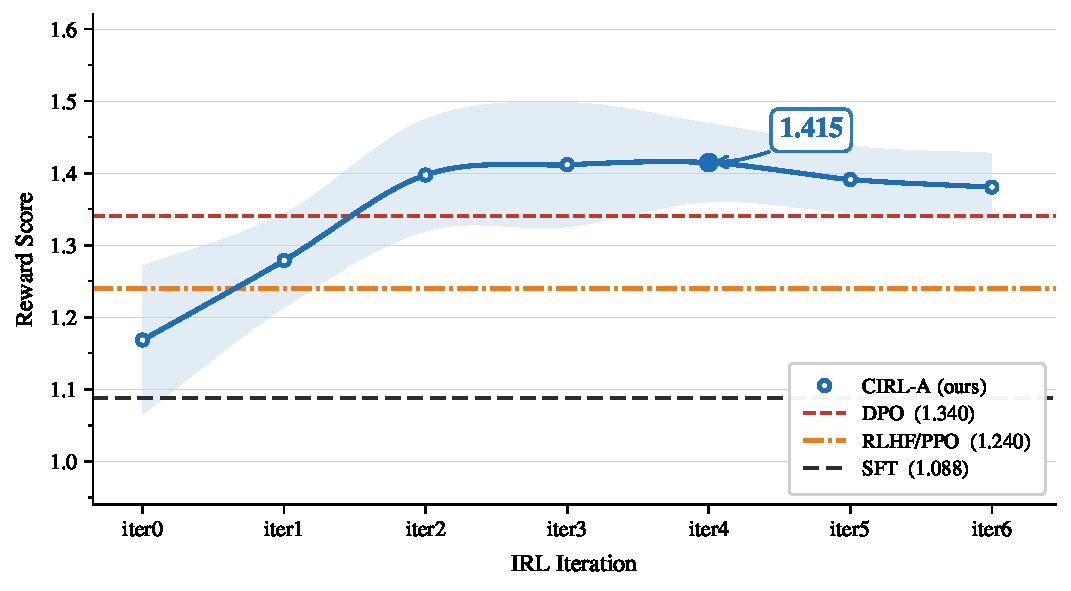
\includegraphics[width=0.88\textwidth]{figures/tldr_reward_curve.pdf}
    \caption{CIRL-A在TL;DR任务上各IRL迭代轮次奖励评分收敛曲线（均值±标准差，4种子）}
    \label{fig:tldr_reward_curve}
\end{figure}

\begin{table}[htbp]
    \centering
    \caption{CIRL-A各IRL迭代轮次奖励评分（TL;DR任务，4种子均值 $\pm$ 标准差）}
    \label{tab:iter_reward}
    \small
    \renewcommand{\arraystretch}{1.2}
    \begin{tabular}{cccccccc}
        \toprule
        & \textbf{iter0} & \textbf{iter1} & \textbf{iter2} & \textbf{iter3} & \textbf{iter4} & \textbf{iter5} & \textbf{iter6} \\
        \midrule
        均值 & 1.169 & 1.279 & 1.398 & 1.412 & \textbf{1.415} & 1.391 & 1.381 \\
        标准差 & 0.103 & 0.065 & 0.078 & 0.086 & \textbf{0.054} & 0.046 & 0.047 \\
        \bottomrule
    \end{tabular}
\end{table}

由表~\ref{tab:iter_reward}可见，CIRL-A的奖励评分随IRL迭代单调提升，从iter0的$1.169$经三轮迭代快速收敛至iter3--4的$1.41$平台区域，iter4达到峰值$1.415 \pm 0.054$，此后iter5--6轻微回落并趋于稳定。这一"快速上升—平台—微降"的三阶段收敛模式与第三章改进下界定理的理论预测相吻合：约束机制在前期允许较大更新步长以快速逼近最优，在平台区自动收紧约束以维持稳定，避免过度优化导致的性能崩溃。

在每轮IRL迭代内部，奖励评分随PPO步数（step0$\to$step390）同样呈现单调上升趋势，表明奖励函数与策略的交替优化在每轮内均能有效推进策略性能。以表现最佳的seed2026为例，iter3内奖励评分从step0的$1.509$平滑提升至step390的$1.522$，期间无明显振荡，训练稳定性良好。

4个随机种子的评分标准差随迭代推进逐步收窄：iter0标准差为$0.103$，iter4--6稳定在$0.046$--$0.054$之间，说明CIRL-A随训练深入产生了越来越稳定的收敛行为，约束机制有效抑制了不同随机轨迹间的发散，使训练行为更具可重复性。

\section{UltraFeedback通用指令跟随实验}

\subsection{主实验结果}

表~\ref{tab:uf_main}报告了各方法在UltraFeedback任务上的最佳checkpoint评测结果（按Avg(8)选择），表~\ref{tab:uf_detail}给出各方法全部迭代轮次的8维度明细。IRL基线的迭代轮次在表中记为r1--r3，与IRL-GRPO的轮次编号对齐。

\begin{table}[htbp]
    \centering
    \caption{UltraFeedback任务主实验结果（Turn~1，各方法最佳checkpoint，MTBench评分，满分10分）}
    \label{tab:uf_main}
    \small
    \renewcommand{\arraystretch}{1.3}
    \setlength{\tabcolsep}{4pt}
    \begin{tabular}{llccccccccc}
        \toprule
        \textbf{方法} & \textbf{ckpt} & \textbf{Writing} & \textbf{Roleplay} & \textbf{Reasoning} & \textbf{Math} & \textbf{Coding} & \textbf{Extract} & \textbf{STEM} & \textbf{Human.} & \textbf{Avg(8)} \\
        \midrule
        SFT           & —  & 6.38 & 6.00 & 6.41 & \textbf{9.58} & 7.33 & 7.80 & 7.78 & 7.08 & 7.29 \\
        DPO\cite{rafailov2023direct} & —  & 6.30 & 5.60 & 6.49 & 9.62 & \textbf{8.18} & \textbf{8.00} & 7.98 & 6.47 & 7.33 \\
        IRL基线\cite{zeng2025d2r}    & r1 & \textbf{6.65} & 6.03 & 6.53 & 9.60 & 7.92 & 7.75 & 7.88 & \textbf{7.30} & 7.46 \\
        \textbf{IRL-GRPO（本文）}    & r2 & 6.45 & \textbf{6.40} & \textbf{7.73} & 9.15 & 7.40 & 7.87 & \textbf{8.18} & 7.08 & \textbf{7.53} \\
        \bottomrule
    \end{tabular}
\end{table}

\begin{table}[htbp]
    \centering
    \caption{UltraFeedback任务全部checkpoint明细（Turn~1，MTBench评分）}
    \label{tab:uf_detail}
    \small
    \renewcommand{\arraystretch}{1.3}
    \setlength{\tabcolsep}{4pt}
    \begin{tabular}{lccccccc}
        \toprule
        \textbf{Metric} & \textbf{SFT} & \textbf{DPO} & \textbf{IRL-base r1} & \textbf{IRL-base r2} & \textbf{IRL-base r3} & \textbf{IRL-GRPO r1} & \textbf{IRL-GRPO r2} & \textbf{IRL-GRPO r3} \\
        \midrule
        Writing     & 6.38 & 6.30 & \textbf{6.65} & 6.58 & 6.60 & 6.22 & 6.45 & 6.50 \\
        Roleplay    & 6.00 & 5.60 & 6.03 & 5.85 & 5.97 & 5.95 & \textbf{6.40} & 6.33 \\
        Reasoning   & 6.41 & 6.49 & 6.53 & 6.48 & 6.21 & 7.05 & \textbf{7.73} & 6.85 \\
        Math        & 9.58 & \textbf{9.62} & 9.60 & 9.12 & 9.50 & 9.18 & 9.15 & 9.25 \\
        Coding      & 7.33 & \textbf{8.18} & 7.92 & 7.48 & 7.20 & 7.58 & 7.40 & 7.66 \\
        Extraction  & 7.80 & 8.00 & 7.75 & 7.75 & 7.82 & 7.98 & 7.87 & \textbf{8.18} \\
        STEM        & 7.78 & 7.98 & 7.88 & 7.82 & 7.85 & 7.95 & \textbf{8.18} & 7.97 \\
        Humanities  & 7.08 & 6.47 & \textbf{7.30} & 6.97 & 6.70 & 6.72 & 7.08 & 6.90 \\
        \midrule
        Avg(8)      & 7.29 & 7.33 & 7.46 & 7.26 & 7.27 & 7.33 & \textbf{7.53} & 7.46 \\
        \bottomrule
    \end{tabular}
\end{table}

\subsection{结果分析}

从主表（表~\ref{tab:uf_main}）可见，IRL-GRPO（本文方法）在最佳checkpoint（r2）上以Avg(8)=$7.53$超越所有基线，相较IRL基线最佳（$7.46$）提升$0.07$分，相较DPO（$7.33$）提升$0.20$分，相较SFT（$7.29$）提升$0.24$分。

从维度分布来看，IRL-GRPO的提升集中于\textbf{推理}（$+1.20$，相较SFT）与\textbf{STEM}（$+0.40$）两个需要深层逻辑推导的维度，Roleplay亦略有提升；而在Math和Coding维度上低于DPO，这与GRPO在语言生成任务上倾向于探索多样性、而在格式严格的代码和数学题上稳定性略弱的特点一致。值得注意的是，IRL基线（D2R）在Writing和Humanities维度上表现最优，说明原始IRL框架在风格化生成上具有一定优势，而IRL-GRPO在这两个维度略有让步以换取推理和STEM的显著增益。

从全部checkpoint明细（表~\ref{tab:uf_detail}）来看，IRL-GRPO在r1至r2间Avg(8)从$7.33$跃升至$7.53$，r3回落至$7.46$，呈现与TL;DR实验一致的"上升—峰值—微降"收敛模式，印证了RMSD约束在多轮IRL迭代中对奖励尺度膨胀的抑制效果在不同模型规模和任务类型上具有普遍性。IRL基线则在r2出现明显下滑（$7.26$），至r3才部分恢复（$7.27$），说明无约束的IRL迭代在第二轮存在不稳定性，与本文理论分析相吻合。

\section{本章小结}

本章在两个任务上对所提方法进行了系统评测。在TL;DR摘要生成任务上，以Pythia-1B为策略底座，CIRL-A在iter4达到峰值奖励评分$1.415 \pm 0.054$，相较RLHF/PPO提升约$14.1\%$，训练动态表现出"快速上升—平台—微降"的三阶段收敛模式，4个随机种子的标准差随迭代从$0.103$收窄至$0.054$，验证了RMSD约束对训练稳定性的关键作用。在UltraFeedback通用指令跟随任务上，以Qwen3.5-9B为底座，IRL-GRPO（r2）以MTBench Avg(8)=$7.53$超越SFT（$7.29$）、DPO（$7.33$）与IRL基线（$7.46$），在推理和STEM维度取得显著增益，且同样呈现稳定的迭代收敛行为。两组实验从不同模型规模和任务类型两个维度，共同印证了第三章改进下界定理关于约束必要性的理论论断，并验证了所提方法的有效性与跨任务泛化能力。
